\documentclass[pdflatex,sn-basic]{sn-jnl}
%%\documentclass[pdflatex,sn-mathphys-ay]{sn-jnl}% Math and Physical Sciences Author Year Reference Style
%%\documentclass[pdflatex,sn-aps]{sn-jnl}% American Physical Society (APS) Reference Style
%%\documentclass[pdflatex,sn-vancouver-num]{sn-jnl}% Vancouver Numbered Reference Style
%%\documentclass[pdflatex,sn-vancouver-ay]{sn-jnl}% Vancouver Author Year Reference Style
%%\documentclass[pdflatex,sn-apa]{sn-jnl}% APA Reference Style
%%\documentclass[pdflatex,sn-chicago]{sn-jnl}% Chicago-based Humanities Reference Style

%%%% Standard Packages
%%<additional latex packages if required can be included here>

\usepackage{graphicx}%
\usepackage{multirow}%
\usepackage{amsmath,amssymb,amsfonts}%
\usepackage{booktabs,tabularx,array,multirow}
\usepackage{amsthm}%
\usepackage{mathrsfs}%
\usepackage[title]{appendix}%
\usepackage{xcolor}%
\usepackage{textcomp}%
\usepackage{manyfoot}%
\usepackage{booktabs}%
\usepackage{algorithm}%
\usepackage{algorithmicx}%
\usepackage{algpseudocode}%
\usepackage{listings}%
\usepackage{booktabs}%
\usepackage{graphicx}%
\usepackage{tikz}
\usetikzlibrary{mindmap,trees,shadows}
%%%%

%%%%%=============================================================================%%%%
%%%%  Remarks: This template is provided to aid authors with the preparation
%%%%  of original research articles intended for submission to journals published 
%%%%  by Springer Nature. The guidance has been prepared in partnership with 
%%%%  production teams to conform to Springer Nature technical requirements. 
%%%%  Editorial and presentation requirements differ among journal portfolios and 
%%%%  research disciplines. You may find sections in this template are irrelevant 
%%%%  to your work and are empowered to omit any such section if allowed by the 
%%%%  journal you intend to submit to. The submission guidelines and policies 
%%%%  of the journal take precedence. A detailed User Manual is available in the 
%%%%  template package for technical guidance.
%%%%%=============================================================================%%%%

%% as per the requirement new theorem styles can be included as shown below
\theoremstyle{thmstyleone}%
\newtheorem{theorem}{Theorem}%  meant for continuous numbers
%%\newtheorem{theorem}{Theorem}[section]% meant for sectionwise numbers
%% optional argument [theorem] produces theorem numbering sequence instead of independent numbers for Proposition
\newtheorem{proposition}[theorem]{Proposition}% 
%%\newtheorem{proposition}{Proposition}% to get separate numbers for theorem and proposition etc.

\theoremstyle{thmstyletwo}%
\newtheorem{example}{Example}%
\newtheorem{remark}{Remark}%

\theoremstyle{thmstylethree}%
\newtheorem{definition}{Definition}%

\raggedbottom
%%\unnumbered% uncomment this for unnumbered level heads

\hypersetup{hypertexnames=false}
\renewcommand{\thetable}{S\arabic{table}}
\renewcommand{\thefigure}{S\arabic{figure}}
\begin{document}

\title[Additional file 1]{Additional file 1: Supplementary tables and figures for ``HANFIS: A Hierarchical Adaptive Neuro-Fuzzy Inference System for Evidence-Based Dynamic Cybersecurity Risk Scoring in Cloud-Native Kubernetes Deployments''}

\author*[1]{\fnm{Mohammad Hafiz} \sur{Hersyah}}\email{mohammadhafizhersyah02@it.unand.ac.id}

\author[2]{\fnm{Derisma} \sur{Derisma}}\email{derisma@it.unand.ac.id}
 

\author[1]{\fnm{Budi} \sur{Rahmadya}}\email{budi-r@it.unand.ac.id}


\affil*[1]{\orgdiv{Computer Engineering Department}, \orgname{Andalas University}, \orgaddress{\street{Kampus Limau Manis Street}, \city{Padang}, \postcode{25162}, \state{West Sumatera}, \country{Indonesia}}}

\affil[2]{\orgdiv{Informatics Department}, \orgname{Andalas University}, \orgaddress{\street{Kampus Limau Manis Street}, \city{Padang}, \postcode{25162}, \state{West Sumatera}, \country{Indonesia}}}

 

\abstract{Supplementary tables and figures moved out of the main text to shorten it. Each item keeps its original caption and values.}

\maketitle

\section*{Supplementary tables}
\begin{table*}[t]
\caption{Experimental preparation, acceptance criteria, and methodological purpose.}
\label{tab1}
\centering
\small
\begin{tabularx}{\textwidth}{@{}p{2.6cm}p{3.4cm}X p{2.4cm}@{}}
\toprule
\textbf{Preparation element} & \textbf{Acceptance criterion} & \textbf{Methodological purpose} & \textbf{Evidence (Runs~7--16)} \\
\midrule
Cluster health & Two Kubernetes nodes in Ready state & Excludes measurements obtained during node degradation or loss of schedulability & Gate passed in all ten pairs \\
Baseline workload P0 & Two of two replicas Ready & Holds application capacity constant across monitoring conditions & Gate passed in all ten pairs \\
Service health & Internal HTTP response code 200 & Confirms that the measurement target remains operational before and after state transitions & Gate passed in all ten pairs \\
Monitoring ON state & Five of five pods Running and fully Ready; Prometheus 1/1 Ready & Defines a complete observability treatment rather than a partially deployed stack & Gate passed in all ten pairs \\
Monitoring OFF state & Zero monitoring pods remaining & Defines a valid control condition without residual collector workloads & Gate passed in all ten pairs \\
Protocol freeze & Scripts, controller definitions, services, system fingerprint, and replication plan present & Prevents unrecorded procedural drift between runs & Applied to Runs~7--16; two aborted attempts logged as incidents \\
Integrity control & SHA-256 manifests validate without mismatch & Detects post hoc alteration or corruption of experimental artefacts & SHA-256 manifest retained for each of the ten run archives \\
Counterbalancing & Prespecified ON--OFF or OFF--ON order & Reduces order, warm-up, cache, and time-dependent bias & Five ON--OFF and five OFF--ON pairs \\
\bottomrule
\end{tabularx}
\end{table*}

\begin{table}[h]
\caption{E1 ablation: membership family $\times$ monotonicity, 5 seeds per cell.}\label{tab:e1-ablation}
\begin{tabular}{@{}llcccc@{}}
\toprule
Scenario & MF family & Monotone & Params. & RMSE (mean $\pm$ SD) & $R^2$ (mean) \\
\midrule
S1 (smooth)     & Gauss   & no  & 176 & $0.093\pm0.021$ & 1.000 \\
S1 (smooth)     & Gauss   & yes & 176 & $0.411\pm0.246$ & 0.999 \\
S1 (smooth)     & Ruspini & no  & 147 & $0.043\pm0.052$ & 1.000 \\
S1 (smooth)     & Ruspini & yes & 147 & $0.073\pm0.066$ & 1.000 \\
S2 (threshold)  & Gauss   & no  & 176 & $0.117\pm0.034$ & 1.000 \\
S2 (threshold)  & Gauss   & yes & 176 & $6.067\pm1.524$ & 0.879 \\
S2 (threshold)  & Ruspini & no  & 147 & $0.646\pm0.051$ & 0.999 \\
S2 (threshold)  & Ruspini & yes & 147 & $2.126\pm0.906$ & 0.983 \\
\botrule
\end{tabular}
\end{table}

\begin{table}[h]
\caption{Post hoc sensitivity of the confirmatory comparison to the EPSS model change: full run versus weeks
whose labels all pre-date 2026-06-15 (skill score, 95\% group-clustered bootstrap CI).}\label{tab:e4-epss}
\begin{tabular}{@{}llcc@{}}
\toprule
Hypothesis & Comparator & Full run & Pre-change weeks \\
\midrule
H1a & Single CVSS score & 0.967 [0.951, 0.980] & 0.973 [0.939, 0.991] \\
H1b & Persistence (4-week) & 0.015 [$-$0.607, 0.246] & $-$0.055 [$-$2.731, 0.201] \\
H1c & Ridge, 7 inputs & 0.696 [0.527, 0.816] & 0.728 [0.484, 0.901] \\
H2 & FlatANFISMatched & 0.665 [0.269, 0.844] & 0.913 [0.753, 0.974] \\
H2$'$ & Flat ANFIS (full) & 0.253 & 0.441 \\
\botrule
\end{tabular}
\end{table}

\begin{table}[ht]
\caption{Explanation-fidelity checks on the 25 saved models. Pairs are the positive-control images P0-IF with and without the active filter; $S^{+}$ denotes the 23 weeks in which exploitability differs between the two.}\label{tab:e6}
\begin{tabular}{@{}p{0.25\linewidth}p{0.29\linewidth}p{0.20\linewidth}l@{}}
\hline
Check & Criterion & Result & Outcome\\
\hline
H6-0 trace vs.\ inference & $|\Delta|\le10^{-9}$, all test rows & 0 & pass\\
H6-neg identical inputs & $|\Delta|\le10^{-9}$, 34 weeks $\times$ 25 models & 0 & pass\\
H6a direction (monotone) & $\hat y_{\mathrm{on}}-\hat y_{\mathrm{off}}\ge-10^{-9}$ on $S^{+}$ & minimum 0 & pass\\
H6b panel structure & panel E unchanged, panel V changes & $0$ and $2.9\times10^{-4}$ & pass\\
H6c deletion test & ratio $\ge2$ and proportion $\ge0.90$ & 4.11 and 0.835 & fail\\
\hline
\end{tabular}
\end{table}

\begin{table}[ht]
\caption{Weekly ranking utility (E15, post hoc): mean over weeks of the Spearman correlation between predicted score and realised label, and precision at the top 20\%.}\label{tab:e15}
\small
\begin{tabular}{@{}p{0.40\linewidth}rrr@{}}
\hline
Horizon and metric & Formula & HANFIS & Persistence\\
\hline
4 weeks (45 weeks): Spearman & 0.994 & 0.969 & 0.992\\
4 weeks: precision at top 20\% & 0.969 & 0.973 & 0.969\\
8 weeks (37 weeks): Spearman & 0.989 & 0.963 & 0.982\\
8 weeks: precision at top 20\% & 0.957 & 0.957 & 0.941\\
12 weeks (29 weeks): Spearman & 0.974 & 0.951 & 0.964\\
12 weeks: precision at top 20\% & 0.924 & 0.952 & 0.883\\
\hline
\end{tabular}
\end{table}

\begin{table}[ht]
\caption{Paired weekly differences in ranking utility (E15, post hoc); 95\% week-bootstrap intervals in brackets.}\label{tab:e15d}
\footnotesize
\begin{tabular}{@{}p{0.30\linewidth}rr@{}}
\hline
Comparison & $\Delta$ Spearman & $\Delta$ precision at top 20\%\\
\hline
4 w: formula $-$ persistence & $+0.002$ $[0.001,\,0.004]$ & $0.000$ $[-0.013,\,0.013]$\\
4 w: HANFIS $-$ persistence & $-0.023$ $[-0.027,\,-0.018]$ & $+0.004$ $[-0.009,\,0.018]$\\
4 w: formula $-$ HANFIS & $+0.025$ $[0.021,\,0.029]$ & $-0.004$ $[-0.013,\,0.000]$\\
8 w: formula $-$ persistence & $+0.007$ $[0.004,\,0.012]$ & $+0.016$ $[0.000,\,0.032]$\\
8 w: HANFIS $-$ persistence & $-0.018$ $[-0.026,\,-0.011]$ & $+0.016$ $[0.000,\,0.032]$\\
8 w: formula $-$ HANFIS & $+0.026$ $[0.020,\,0.031]$ & $0.000$ $[0.000,\,0.000]$\\
12 w: formula $-$ persistence & $+0.010$ $[0.005,\,0.017]$ & $+0.041$ $[0.014,\,0.076]$\\
12 w: HANFIS $-$ persistence & $-0.013$ $[-0.025,\,-0.002]$ & $+0.069$ $[0.034,\,0.103]$\\
12 w: formula $-$ HANFIS & $+0.024$ $[0.017,\,0.032]$ & $-0.028$ $[-0.055,\,-0.007]$\\
\hline
\end{tabular}
\end{table}

\begin{table}[ht]
\caption{Input-change strata at four weeks (E16, post hoc): rows, mean squared error (persistence / formula / HANFIS), and skill against persistence with 95\% intervals.}\label{tab:e16}
\footnotesize
\setlength{\tabcolsep}{3pt}
\begin{tabular}{@{}p{0.17\linewidth}rp{0.19\linewidth}p{0.22\linewidth}p{0.23\linewidth}@{}}
\hline
Stratum & Rows & MSE & Skill, formula & Skill, HANFIS\\
\hline
Input changed & 628 & 0.637 / 0.382 / 0.557 & $0.400$ $[0.308,\,0.487]$ & $0.125$ $[-0.402,\,0.333]$\\
No input change & 452 & 0.107 / 0.106 / 0.202 & $0.002$ $[-0.069,\,0.037]$ & $-0.900$ $[-4.171,\,-0.206]$\\
\hline
\end{tabular}
\end{table}

\begin{table}[ht]
\caption{Calibration of four-week out-of-fold predictions (E21, post hoc). Mean error (prediction minus label), and slope $\beta$ and intercept $\alpha$ of the regression of the label on the prediction, with 95\% image-bootstrap intervals. Unaffected rows are those whose label window does not straddle the change of the EPSS model.}\label{tab:e21}
\footnotesize
\setlength{\tabcolsep}{3pt}
\begin{tabular}{@{}p{0.17\linewidth}p{0.26\linewidth}p{0.26\linewidth}p{0.26\linewidth}@{}}
\hline
Predictor & Mean error & Slope $\beta$ & Intercept $\alpha$\\
\hline
\multicolumn{4}{@{}l}{\emph{All rows (1080)}}\\
Persistence & $-0.097$ $[-0.196,\,-0.013]$ & $0.997$ $[0.986,\,1.007]$ & $0.109$ $[0.012,\,0.228]$\\
Formula & $-0.040$ $[-0.106,\,0.017]$ & $0.998$ $[0.990,\,1.005]$ & $0.048$ $[-0.021,\,0.132]$\\
HANFIS & $0.016$ $[-0.080,\,0.104]$ & $1.025$ $[1.008,\,1.044]$ & $-0.115$ $[-0.228,\,0.007]$\\
\multicolumn{4}{@{}l}{\emph{Unaffected rows (890)}}\\
Persistence & $-0.015$ $[-0.079,\,0.025]$ & $0.997$ $[0.993,\,1.001]$ & $0.026$ $[-0.017,\,0.091]$\\
Formula & $0.012$ $[-0.029,\,0.040]$ & $1.000$ $[0.997,\,1.002]$ & $-0.012$ $[-0.044,\,0.035]$\\
HANFIS & $0.068$ $[-0.029,\,0.157]$ & $1.031$ $[1.014,\,1.053]$ & $-0.193$ $[-0.300,\,-0.085]$\\
\hline
\end{tabular}
\end{table}

\section*{Supplementary figures}
\begin{figure*}[t]
\centering
\resizebox{\textwidth}{!}{%
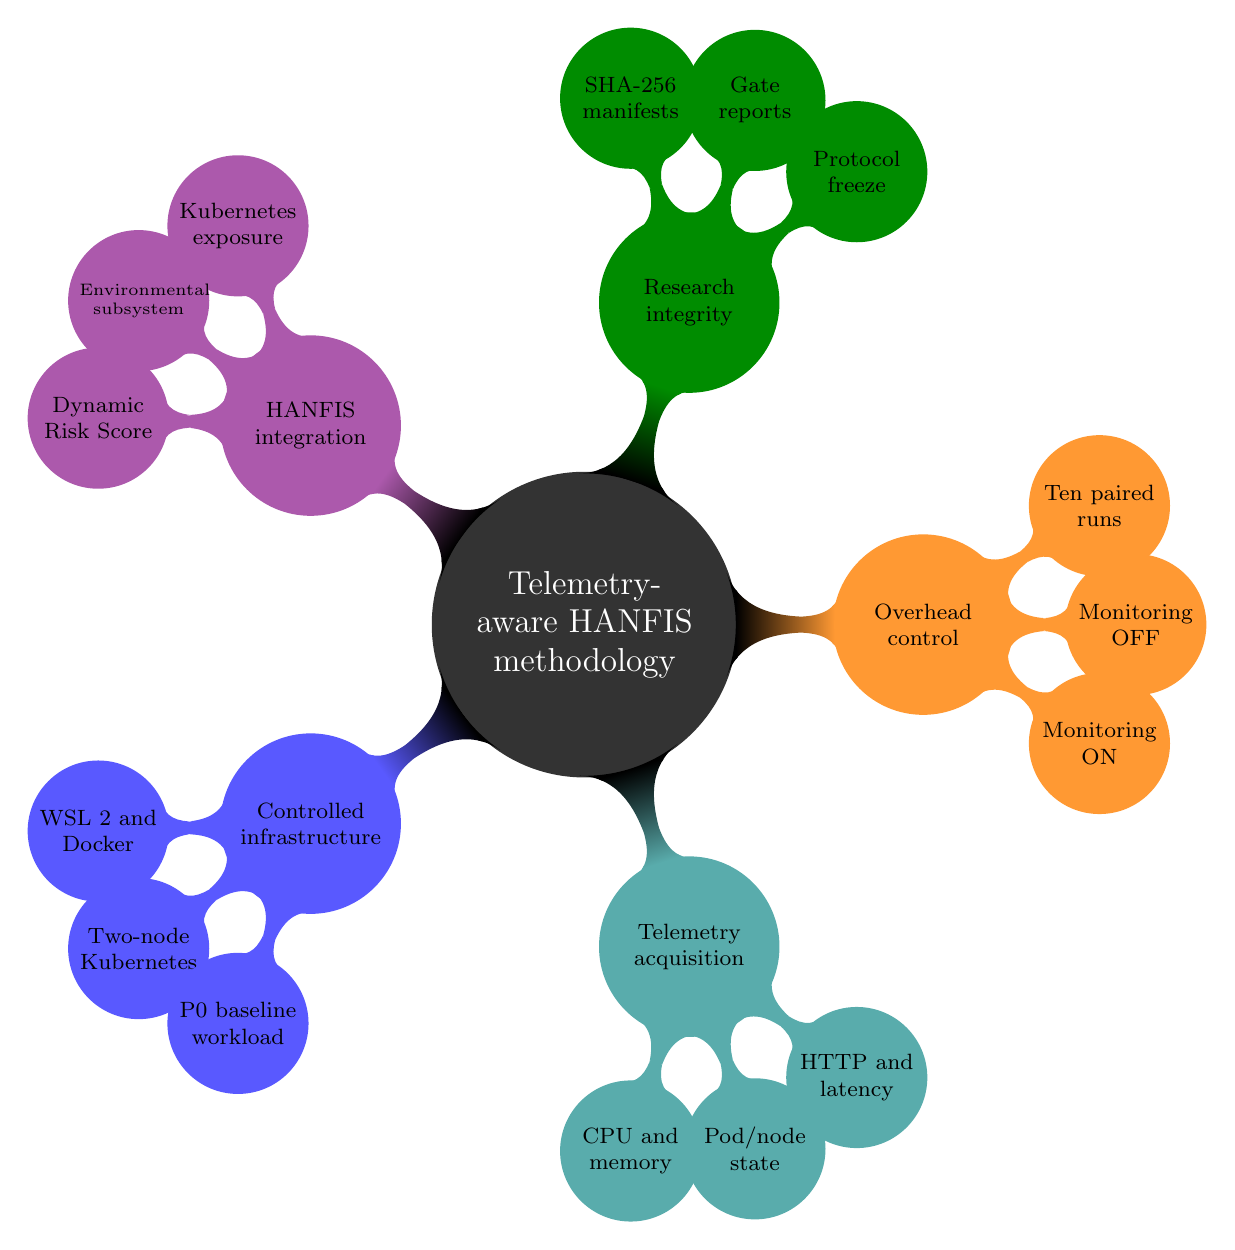
\begin{tikzpicture}[
  mindmap,
  grow cyclic,
  every node/.style={concept, font=\footnotesize, align=center},
  root concept/.append style={concept color=black!80, text=white, minimum size=2.8cm},
  level 1/.append style={level distance=4.3cm, sibling angle=72},
  level 2/.append style={level distance=2.7cm, sibling angle=34},
  infrastructure/.style={concept color=blue!65},
  measurement/.style={concept color=teal!65},
  validation/.style={concept color=orange!80},
  model/.style={concept color=violet!65},
  evidence/.style={concept color=green!55!black}
]
\node[root concept]{Telemetry-aware HANFIS methodology}
 child[infrastructure]{node{Controlled infrastructure}
   child{node{WSL 2 and Docker}}
   child{node{Two-node Kubernetes}}
   child{node{P0 baseline workload}}}
 child[measurement]{node{Telemetry acquisition}
   child{node{CPU and memory}}
   child{node{Pod/node state}}
   child{node{HTTP and latency}}}
 child[validation]{node{Overhead control}
   child{node{Monitoring ON}}
   child{node{Monitoring OFF}}
   child{node{Ten paired runs}}}
 child[evidence]{node{Research integrity}
   child{node{Protocol freeze}}
   child{node{Gate reports}}
   child{node{SHA-256 manifests}}}
 child[model]{node{HANFIS integration}
   child{node{Kubernetes exposure}}
   child{node[font=\fontsize{6.2}{7}\selectfont]{Environmental subsystem}}
   child{node{Dynamic Risk Score}}};
\end{tikzpicture}}

\caption{Methodological mind map linking the cloud-native testbed, telemetry acquisition, monitoring-overhead controls, reproducibility evidence, and HANFIS integration.}
\label{fig:methodology-mindmap}
\end{figure*}

\begin{figure}[h]
\centering
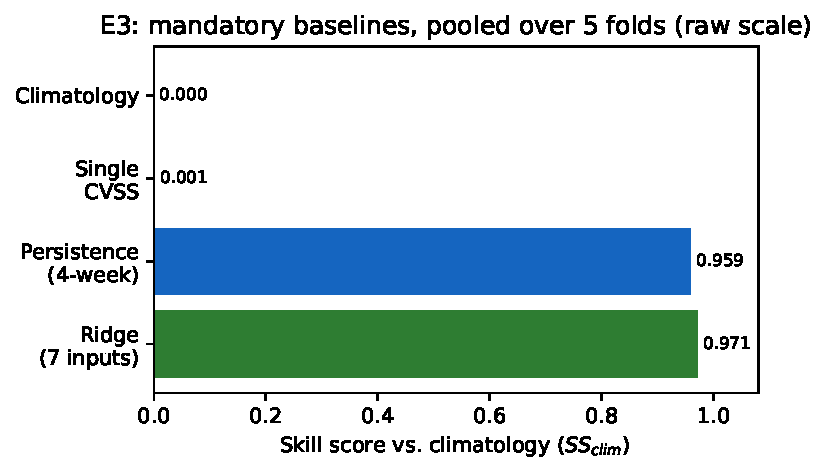
\includegraphics[width=0.75\linewidth]{fig_e3_baselines.pdf}
\caption{Mandatory baselines' skill against climatology, pooled over 5 folds. A single CVSS score
now adds modest skill over climatology (22\%, up from essentially nothing on the earlier 27-image
pilot); persistence and ridge separately recover over 90\% of the climatology-relative skill each, though not of each other; see the mandatory-baselines table in the main text for the reversal in their relative standing.}\label{fig:e3-baselines}
\end{figure}

\begin{figure}[h]
\centering
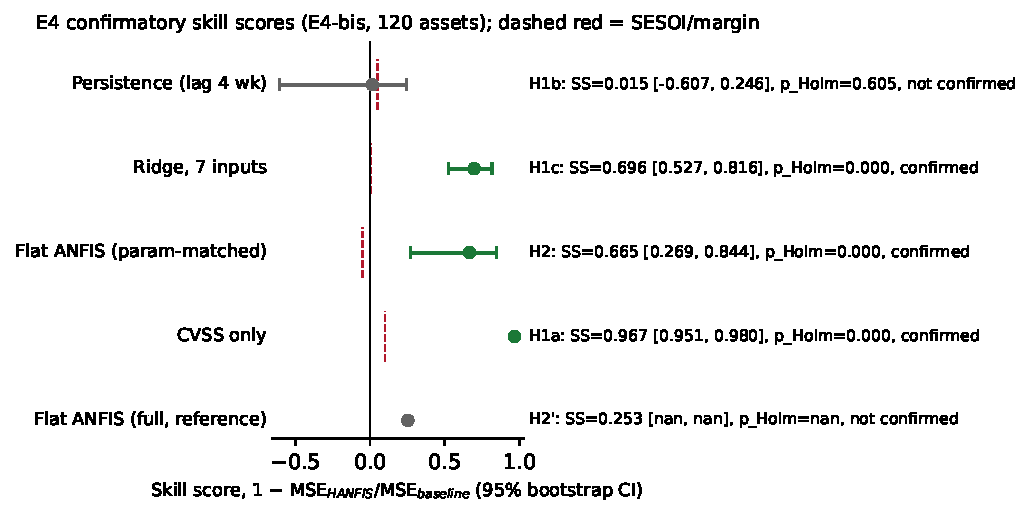
\includegraphics[width=0.78\linewidth]{fig_e4_skill_scores.pdf}
\caption{E4 confirmatory results: HANFIS skill score against each comparator with 95\% group-clustered
bootstrap confidence intervals. Green bars exclude zero (confirmed); the red bar (H1b, vs.\ persistence)
does not.}\label{fig:e4-skill-scores}
\end{figure}

\end{document}
